% Preamble =====================================================================
\documentclass{article}

% Allow special characters, and additional commands such as `\FloatBarrier`
\usepackage[utf8]{inputenc}
\usepackage[section]{placeins}

% Allow syntax highlighting of source code (requires shell-escape flag)
\usepackage{minted}

% Allow images, and set them to import from the "./images" directory
\usepackage{graphicx}
\graphicspath{ {./images/} }
% Set the dimensions of the paper to render on
\usepackage{geometry}
\geometry{a4paper, total={170mm,257mm}, left=20mm, top=20mm,}
% Colour in references, such as hyperlinks
\usepackage{hyperref}
\hypersetup{colorlinks=true, linkcolor=black, filecolor=magenta, urlcolor=blue,
    citecolor=black}


% Document =====================================================================
\begin{document}


\begin{titlepage}
    \vspace*{\fill}
    \begin{center}
        \Huge\textbf{What are computer protocols, how are they verified against attacks, and how is this relevant to people today?}\\
        \huge\textit{Edmund Goodman}\\
        \huge\textit{August 2017 / May 2021}
    \end{center}
    \vspace*{\fill}
\end{titlepage}

\section{Abstract}


% Add a table of contents section to the table of contents
\addtocounter{section}{1}
\addcontentsline{toc}{section}{\protect\numberline{\thesection} Contents}
\tableofcontents


\section{Introduction}
\subsection{Security}
In 1997 Tim Berners-Lee wrote a research paper ‘Realising the Full Potential of
the Web’. In it, he said “The web was designed as an instrument to prevent
misunderstanding”. This is, in hindsight, clearly false. Most weeks we hear a
news report of hackers  stealing state and corporate secrets and causing
millions of pounds in damages and hundreds of thousands in fines. Bugs such as
Heartbleed and Cloudleak have destroyed companies, and damaged the
livelihoods of many hundreds of people. This is an issue of computer security,
which is only indirectly in the public eye, but is hugely important.  This is
why computer protocols are relevant today, companies lose money and people lose
personally identifiable information, because someone has uncovered an exploit
and used it to their advantage.

\subsection{Technique}
In this essay I set out to investigate how computer protocols, specifically
authentication protocols, work, how and why they are attacked, and whether this
is still relevant, given that a lot of research on the topic was done around
forty years ago. I decided to read research papers by contemporary computer
scientists, who were on the cutting edge of research, and try to write a program
to emulate one of the protocols running.

\subsection{Why are protocols important?}
Computer protocols are intrinsically related to security, as anything wrong with
them can lead to catastrophic security breaches, that could affect innumerable
numbers of systems and machines. Firstly I will discuss what computer protocols
are, and look over a variety of types of protocol, and will then take a more in
depth look at authentication protocols, especially the Needham-Schroeder
protocol, is a good example of protocols of the authentication variety, and has
a freshness flaw, that links well into my second question: how are protocols
verified against attacks? I will then go over a variety of contemporary
techniques of verification. Finally, I will analyse how relevant protocols are
today, with a similar focus on authentication protocols.

\section{What are computer protocols?}
\subsection{Types of protocols}
In the loosest sense, a computer protocol is “A sequence of operations that
ensure protection of data”  one could consider the analogy - the recipe a
computer follows to bake a cake. However, they come in many types, each of which
achieves a different thing. Consensus protocols, ensure that even if a
proportion of a system fails, the system keeps going and maintains integrity.
This type of protocol is used in the real world very commonly, but like most of
this topic, is relatively unknown. Consensus protocols are used for things like
clock synchronization - which is incredibly important in the real world, as
unsynchronized clocks can cause huge problems in transport systems. Even the
algorithms search engine conglomerates like Google uses to order pages are
heavily reliant on consensus protocols. Cryptographic protocols are designed to
take data, and encrypt it, making it unreadable, usually to prevent unauthorised
access. Cryptographic protocols can be ‘symmetric’, requiring the same
encryption key to encrypt and decrypt, or ‘asymmetric’, requiring linked, but
different, encryption keys to encrypt and decrypt. They are used ubiquitously
and commonly, from your smartphone to in top-secret government organisations,
and are a founding pillar of computer security. Transport protocols, as the name
suggests, ensure that data is transferred securely. This type of protocol is
generally used for things like secure browsing on the internet, and to stop
other people reading your emails and SMS messages. If this type of protocol has
a vulnerability, swathes of personally identifiable information can be lost. The
type of protocol I mostly researched in the course of this essay is an
authentication protocol. An authentication protocol helps two parties establish
a secret - which is in most cases an encryption key, that they both trust. This
is hugely important, and is the backbone of many security systems, as
establishing a secret between two parties is the basis for many transport
protocols, discussed above.

\subsection{How protocols link to security}
Security is in essence what all of these protocols strive to achieve. Security
is especially important in today’s political and sociological climate. Back in
the 1950s when computers were just being developed, security was not an issue.
There were no malicious parties in the teams of computer scientists doing
research - everyone started with a “tabula rasa”, did their research, and reset
the computer. However, as computers got smaller and more widely available, and
LAN and WAN were invented, people realised they could circumvent security
systems. This lead to an arms race - where cryptography, and computer protocols
were invented, to maintain data integrity and security.

\subsection{The Needham-Schroeder protocol}
The task of an authentication protocol at first glance seems impossible, To
share a secret between two parties, when all communications between them can be
heard, but can be done in a remarkable short number of steps. One of the first
teams to achieve this was Roger Needham and Michael Schroeder. In their paper
“Using Encryption for Authentication in large networks of computers” they
outlined a authentication protocol for two parties and an authentication server.
This paper was a foundation for many authentication protocols today.

\subsubsection{What is the Needham-Schroeder protocol}
One of the protocols discussed in the Needham-Schroeder paper aims for the
“Establishment of authenticated and interactive communication between two
principals on different machines”. Broken down, this means creating a two-way
communication, like email or SMS between two different people on two different
computers. To demonstrate how protocols work, computer scientists have devised a
notation that describes authentication protocols. This is the notation as
described in Needham-Schroeder’s paper:

\subsubsection{Protocol notation}
Consider the following protocol:
\begin{equation}
    A \rightarrow AS: A, B, I_{A1}
\end{equation}

\noindent We can break this down by the colon. Before the colon $A \rightarrow AS$ means
the message is from the sender $A$ (commonly personified as Alice) and to the
server $AS$ (commonly personified as Sam). After the colon the $A, B, I_{A1}$ is
the content of the message. The character $I$ (sometimes indicated by $N$)
denotes a nonce (which is shorthand for a number only used once) and the
subscript denoted the sender and the number of the nonce. Nonces are used to
guarantee the freshness of the message.

\medskip

\noindent Consider the following protocol:
\begin{equation}
    A \rightarrow B: \{CK, A\}^{KB}
\end{equation}

\noindent We can similarly break this down by the colon and surmise from our previous
knowledge that it is a message from $A$ (Alice) to $B$ (Bob). The content of the
message however is different. Content within curly braces is encrypted with the
encryption key shown in superscript next to it. Furthermore content with the
character $K$ in tends to stand for encryption key’s. For example, in this case
$CK$ is a conversation key and $KB$ is the key of Bob. Furthermore, we can do
arithmetic operations on nonces, as they are numbers, this will prove useful
later and is denoted by $I_{B1} - 1$.

\medskip

\noindent The Needham-Schroeder protocol is:
% ===== 1 =====
\begin{equation}
    A \rightarrow AS: A, B, I_{A1}
\end{equation}
% ===== 2 =====
\begin{equation}
    As \rightarrow A: \{ I_{A1}, B, CK, \{CK, A\}^{KB} \}^{KA}
\end{equation}
% ===== 3 =====
\begin{equation}
    A \rightarrow B: \{CK, A\}^{KB}
\end{equation}
% ===== 4 =====
\begin{equation}
    B \rightarrow A: \{I_B\}^{CK}
\end{equation}
% ===== 5 =====
\begin{equation}
    A \rightarrow B: \{I_B - 1\}^{CK}
\end{equation}


\noindent This can be shown visually in the diagram:
\begin{figure}[ht]
    \centering
    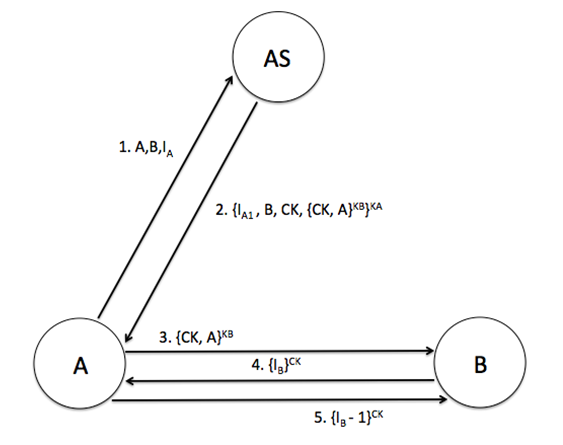
\includegraphics[width=0.6\textwidth]{protocolDiagram.png}
    \caption{A diagram of the steps Needham-Schroeder protocol}
    \label{fig:protocolDiagram}
\end{figure}

Breaking the protocol down now becomes fairly trivial: In step 1, Alice
indicates that she wants to communicate with Bob and provides the nonce
$I_{A1}$. The authentication server then replies with a big package of content
$\{ I_{A1}, B, CK, \{CK, A\}^{KB} \}^{KA}$. Alice then decrypts what she can
(the outer layer of the message) and sends on what she can’t to Bob in step 3.
Then Bob replies with a fresh nonce and Alice responds with the nonce, but
modified by an arithmetic operation, for example subtract 1.


\subsubsection{Computer modelling}
I have written a computer model in the programming language Python  that
endeavours to model computer protocols with the test case of the
Needham-Schroeder protocol, <See appendix 1> This is relevant to this essay
as it is on the topic of computer protocols, but also, it is written in another
fundamental facet of computer science, programming. My computer model takes a
list of commands as an input, and interprets them with standard protocol
notation, It then generates numbers to represent them, and uses rudimentary
encryption where necessary. This produces an output in the form of a table,
containing each of the messages, which gives a better sense of how protocols
work. However, as with any program, it might still contain bugs that hinder its
performance.

\subsubsection{Flaws in the Protocol}
However, there is an issue, which has been rectified in the Kerberos and
Denning-Sacco protocols, but had passed undetected for an extended and
potentially dangerous period of time. This was ironically predicted by Needham
and Schroeder in his commentary on the paper ‘Protocols that are developed here
are prone to extremely subtle errors that are unlikely to be detected in normal
operation.’ This highlights the issue that, in essence, most of computer science
today could be sitting on a metaphoric unexploded bomb. And leads us onto my
next question - how are protocols verified against attacks.

\section{How are protocols verified against attacks}
\subsection{Why do protocols need to be verified?}
The problem computer scientists now faced was they had many authentication
protocols, used widely and in varied contexts, but they didn’t really know if
they were secure. A single exploit on one of these protocols could cripple
telecommunications, and consumer trust in the industry. This caused an agenda
among computer scientists, surmised in the Needham-Schroeder paper as a “need
for techniques to verify the correctness of such protocols”. 11 years later,
Needham co-authored a paper on exactly this with Burrows and Abadi. Titled ‘A
logic of authentication’, this paper outlined a logic for analysing
authentication protocols and then went on to use this technique on a variety of
commonly used protocols.

\subsection{BAN logic}
The technique (BAN logic, shorthand for Burrows-Abadi-Needham logic) rectifies
the ambiguity of the protocol notation, replacing in with a formal logic
notation, then uses this notation to find all assumptions made for the protocol
to work. If there are any dubious assumptions, the protocol might be vulnerable
to exploits. The formal logic uses a notation that was easy to typeset  when the
paper was written, but ironically, with the digital era came ASCII  and UNICODE
, which inhibits the writing of the characters used in the formal logic. In
their paper, Burrows, Abadi and Needham then proceeded to analyse various
protocols for flaws, including: Needham-Schroeder, Otway-Rees, Kerberos,
Wide-mouthed frog, Yahalom, Andrew RPC and CCITT. Exactly half of the protocols
analysed had “Bugs”, which could be exploited with dangerous results

\subsection{Informal techniques}
Furthermore, other computer scientists have devised less formal techniques
protocol designers should follow, that mean protocols are less likely to be
vulnerable to attacks. For example, Ross Anderson and Roger Needham wrote the
paper “Robustness principles for public key protocols”, in which they suggested
various principles, which include:
\begin{enumerate}
    \item
        “Sign before encrypting”. This is important as if you sign after
        encryption, you can be subject to “novel” attacks, where a malicious
        party can forge your signature, furthermore, this is an easy mistake for
        a lazy engineer to make.
    \item
        “Be careful how entities are distinguished”. Entities in this case
        refers to encryption keys, as if you use one encryption key for two
        processes, as not only is it twice as easy to compromise the protocol,
        but various attacks can be derived from it (see principle 4).
    \item
        "Distinguish between different runs of the same protocol”. This is
        involved in stopping replay attacks such as the one that compromised the
        Needham-Schroeder protocol.
    \item
        "Do not assume the secrecy of others secrets”. This idea is mirrored
        many other fields, for example the idiom “Never trust the user”. It is
        fairly trivial to see how others flawed secrets could compromise you.
    \item
        "Do not assume a message has a certain form, unless you can verify it
        does”. This is also fairly self-explanatory, as a misunderstanding of a
        message could be catastrophic to a protocol.
    \item
        "Be explicit about crypto primitives”. Crypto primitives  are basic
        cryptographic algorithms, i.e. hashing  or encryption. This removes
        possible ambiguity among principals, and disallows insecure algorithms
        to be used.
    \item
        "Robust security is about explicitness”. Taking all of the above
        principles into account, the key tenet of building a protocol is to be
        clear.
\end{enumerate}

\subsection{Should new protocols be developed?}
In an informal discussion Gavin Stark (Computer Laboratory, University of
Cambridge) suggested that at this stage, producing new protocols was a bad idea.
Commonly used protocols were written around forty years ago, and have passed the
test of time because they work. Recently, students have been rewriting and
making new protocols, but in doing so, have broken the security strived for in
the first place. Although we have developed mathematical and informal techniques
for verification against attacks, we still cannot perfectly ensure a protocol is
valid.

However, there are naturally new scenarios to which no old protocols are
applicable, so some cases necessitate the writing of new protocols. Whilst this
has the drawback of them not having stood the test of time, more tools to ensure
such protocols are correct (such as BAN logic), and most often the greatest
security issue in a system is incorrect implementation or application of a
protocol, as opposed to it inherently being flawed, so it may be better to
develop a new one, than try to "bodge" an old one into a scenario where it
should not be applied.

\section{How are protocols relevant to people today?}
This field of computer science is, in my opinion, very relevant to people today.
This is due to clear fact that errors do occur, even in the most established
places. This can lead to cataclysmic exploits, that can and will rock companies
and individuals. I have already discussed Heartbleed and Cloudleak as examples,
but there are many (albeit varying in magnitude). Furthermore, it is lesson to
computer scientists now and in the future, there is no substitute for good
logic, and there is no shortage of sloppy and badly written code and logic.
Also, errors in protocols tend to be so intrinsic to platforms using them, there
is a great difficulty in fixing thing them. This links back to the introduction
in that errors in protocols can have terrible results on computer security. Some
might argue that everything in this field happened 40 years ago, and it is thus
dead, but I suggest that its age makes it more important, as it is more likely
to be a basis for more things on more platforms. This means that even if the
protocols are entirely correct, it is probable, someone will implement it in a
way it was not meant for, and that could cause a cascade of effects. Many people
may not need to know about them, but anybody considering a career in computer
science, would do well to have a rudimentary understanding of protocols

\section{Conclusion}
To conclude, in this essay I have answered three questions: what are computer
protocols, how are they verified against attacks, and how is this relevant to
people today. I have investigated computer protocols to be “A sequence of
operations that ensure protection of data”, and I know that they come in various
different varieties, from consensus to transport. I then took an in depth look
at authentication protocols and the literature surrounding them. I have looked
at the methods used to verify these protocols against attacks, considering both
formal and informal techniques. Finally, I considered whether protocols are
relevant to people today, and concluded that anybody following a career in
computer science should definitely find it relevant.

% Add a references section to the contents list
\addtocounter{section}{1}
\addcontentsline{toc}{section}{\protect\numberline{\thesection} References}

% Write out the biobliography in IEEE format, and include uncited references
\bibliographystyle{ieeetr}
\bibliography{references.bib}
\nocite{*}

\section{Glossary}

Authentication protocol - A type of computer protocol, which tries to establish a secure connection between two principals.
Authentication server - A computer whose purpose is to participate in an authentication protocol
Consensus protocols - A type of computer protocol, which tries to ensure that data integrity, even if there is a failure in the system storing it.
Encryption - The process of encoding information, such as text, generally to prevent unauthorised access
Encryption key - A piece of data required for encryption or decryption to occur
Entities - A broad term for distinct part of a protocol i.e. a principal, a nonce, or an encryption key.
Exploit - taking advantage of a flaw in a computer system, typically for malicious purposes.
Freshness - Whether something is new/has not been used before, this is important in preventing replay attacks.
Hackers - a person who uses computers to gain unauthorized access to data.
Hashing - The transformation of text of an arbitrary length, to a fixed length, where a small change in the input would create a large change in the output, algorithms range from the insecure (md5) to the military grade (SHA4096).
Integrity - The accuracy and consistency of data/information
LAN - Local Area Network, a specific type of computer network
Machine - A independent computer, for example a laptop.
Nonce - A number used only once, used to ensure freshness
Parties - A person or people participating in a protocol.
Personally identifiable information - Any information that can be used to distinguish one person from another.
Principal - Similar to a party, A person participating in a protocol.
Replay attack - The re-use of an old run of a protocol to impersonate a principal without knowledge of their key, that should be required.
Signature - The digital equivalent of its namesake, verifies that a principal wrote the message.
Tabula rasa - Literally ‘A blank slate’, if a computer is reset to Tabula rasa, all data is deleted from it.
Transport protocols - A type of computer protocol, which deals with the transportation and security thereof of data.
Trust - Whether it is reasonable for a principal to assume something is true, i.e. the principal trusted that Nonce IB is fresh.
WAN - Wide Area Network, a specific type of computer network        



\newpage
\section{Appendices}
\subsection{Sample run}
\begin{figure}[ht]
    \centering
    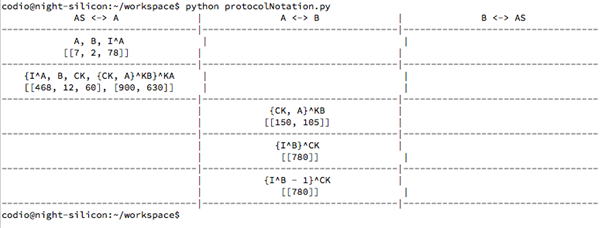
\includegraphics[width=0.75\textwidth]{sampleRun.png}
    \caption{A screenshot of a sample run of the program}
    \label{fig:sampleRun}
\end{figure}

\subsection{Source code}
\begin{minted}{python}
import time
import collections
import random

def chunks(braces):
    """helper function to pair a list up 1st with last, 2nd with
    penultimateetc."""
    newbraces = collections.OrderedDict()
    for i in range(0, int(len(braces)/2)):
        newbraces[braces[i]] = braces[-(i+1)]
    return newbraces

def encrypt(plain, keys):
    """The most basic private key encryption I could think of - the focus is not
    on cryptography #it works by multiplying the key(s) by the plaintext - both
    of which are numerically encoded"""
    superKey, cipher = 1, []
    for n in keys:
        superKey *= n
    for i in plain:
        cipher.append(i*superKey)
    return cipher        

def generateNonce():
    """Note this is NOT a timestamp, but merely a nonce based off the time"""
    #Ensure timestamps do not collide, compromising their use as nonces
    time.sleep(0.1)
    #Remove all zeroes, to eliminate math error
    return int(time.strftime('%S%M%H').replace("0", "")) 

def assignVariables(newMessageParts):
    """Long helper function to make a dictionary of variables, so they can be
    accessed #the sequence of if statements handeles different variable types"""
    message = []
    for newMessagePart in newMessageParts:
        while 1:
            try:
                message.append(variables[newMessagePart])
                break
            except:
                if "I" in newMessagePart:
                    variables[newMessagePart] = generateNonce()
                elif bool(set(["+", "-", "*", "/"]) & set(newMessagePart)):
                    newMessagePart = resolveOperands(newMessagePart)
                    variables[newMessagePart] = newMessagePart
                elif bool(set([str(x) for x in range(0, 3*10**3)]) & set(newMessagePart)):
                    variables[newMessagePart] = int(newMessagePart)
                else:
                    variables[newMessagePart] = random.randint(0, 35)
    return message

def resolveOperands(message):
    """Short helper function to "resolve operands" i.e. do the arithmetic"""
    message = [i for i in message]
    delList = []
    for i in ["+", "-", "*", "/"]:
        for n in range(0, len(message)):
            if message[n] == i:
                delList.append(n)
    for n in delList:
        exec("working = int(message[n-1]){}int(message[n+1])".format(message[n]))
        message.pop(n+1)
        message.pop(n)
        message[n-1] = working
    return message



needhamSchroederConventional2Way = [
    "A -> AS: A, B, I^A",
    "AS -> A: {I^A, B, CK, {CK, A}^KB}^KA",
    "A -> B: {CK, A}^KB",
    "B -> A: {I^B}^CK",
    "A -> B: {I^B - 1}^CK",
]
variables = {}
print("             AS <-> A              |", end="")
print("              A <-> B              |", end="")
print("              B <-> AS")
print("-----------------------------------|------------------", end="")
print("-----------------|-----------------------------------")
for step in needhamSchroederConventional2Way: #evaluate statement
    #Split up command into recipient and command
    command = step.split(": ")
    command[0] = (command[0].split(" -> "))
    recipient = [command[0][0], command[0][1], "public"]
    
    #Find braces so as to evaluate statement
    braces = [i for i, x in enumerate([i for i in command[1]]) if x == "{"]
    braces.extend([i for i, x in enumerate([i for i in command[1]]) if x == "}"])
    braces = chunks(braces)
    
    #Sse the positions of the braces to find the encryption keys and continue
    #cutting up the command
    encryptionKeys, messageParts = [], []
    for k, v in braces.items():
        encryptionKeys.append(command[1][(v+2):(v+4)])  
        messageParts.append(command[1][k:v+1])
    if messageParts == []:
        messageParts.append(command[1])
    if encryptionKeys == []:
        encryptionKeys.append('1')
    
    #Format the command to remove repeats and make linked lists of the 
    #schema (messageParts : encryptionKeys)
    for i in range(1, len(messageParts)):
        if messageParts[i] in messageParts[i-1]:
            startIndex = messageParts[i-1].find(messageParts[i]) - 2
            endIndex = startIndex + len(messageParts[i]) + 5
            messageParts[0] = messageParts[0].split(
                messageParts[0][startIndex:endIndex]
            )
            messageParts = [x for sublist in messageParts for x in sublist]
            messageParts = "".join(messageParts)
            messageParts = messageParts.split("{")[1:]
            messageParts = ["{"+x for x in messageParts]    
    for i in range(0, len(messageParts)):
        if "{" in messageParts[i]:
            messageParts = [l[1:-1] for l in messageParts]
            break
    
    #Assign values to the variables
    concFinalMessage = []
    for e in range(0, len(encryptionKeys)):
        formatEncryptionKeys = [encryptionKeys[i] for i in list(set(
            [ee for ee in range(0, e+1)]
        ))]
        splitMessageParts = messageParts[e].split(", ")
        message = assignVariables(splitMessageParts)
        keys = assignVariables(formatEncryptionKeys)
        finalMessage = encrypt(message, keys)
        concFinalMessage.append(finalMessage)

    #display the generated data in a tabular format
    comLen, mesLen, spaLen = len(command[1]), len(str(concFinalMessage)), 35
    comLen2, mesLen2 = (35-comLen)/2, (35-mesLen)/2
    space, line = spaLen*" ", spaLen*"-"
    com = int(comLen2)*" "+str(command[1])+(int(comLen2)+1)*" "
    mes = int(mesLen2)*" "+str(concFinalMessage)+(int(mesLen2)+1)*" "
    #print(com, mes, space)
    if command[0] == ['A', 'AS'] or command[0] == ['AS', 'A']:
        print("{}|{}|{}\n{}|{}|{}\n{}|{}|{}".format(
            com, space, space, mes, space, space, line, line, line)
        )
    if command[0] == ['A', 'B'] or command[0] == ['B', 'A']:
        print("{}|{}|{}\n{}|{}|{}\n{}|{}|{}".format(
            space, com, space, space, mes, space, line, line, line)
        )
    if command[0] == ['B', 'AS'] or command[0] == ['AS', 'B']:
        print("{}|{}|{}\n{}|{}|{}\n{}|{}|{}".format(
            space, space, com, space, space, mes, line, line, line)
        )

\end{minted}


\end{document}
